\subsection{CA}
Il preventivo della macrofase Customer Acceptance è stato stilato insieme alla decisione del preventivo a finire al termine della macrofase PB riportato alla sezione §6.2.5.4
\subsubsection{Validazione requisiti obbligatori}
\paragraph{Prospetto Orario}
\begin{center}
	\renewcommand{\arraystretch}{1.8} %aumento ampiezza righe
	\begin{tabular}{ |m{10em}|c|c|c|c|c|c|c| }
	\hline
	\textbf{Membro} & \textbf{Re} & \textbf{Am} &  \textbf{An} &  \textbf{Pt} &  \textbf{Pg} &  \textbf{Ve} &  \textbf{Totale}\\
    \hline
    Irene Benetazzo   & - & 1 & - & 1 & - & 5 & \textbf{7} \\
    \hline
    Tommaso Berlaffa  & - & - & - & 2 & 2 & 3 & \textbf{7} \\
    \hline
    Mattia Episcopo   & - & - & - & - & 2 & 5 & \textbf{7} \\
    \hline
    Pietro Macrì      & - & - & - & 1 & 1 & 6 & \textbf{8} \\
    \hline
    Qi Fan Andrea Pan & - & 1 & - & - & 1 & 5 & \textbf{7} \\
    \hline
    Matteo Pillon     & - & - & - & 2 & - & 6 & \textbf{8} \\
    \hline
    Samuele Rizzato   & 2 & 2 & - & - & - & 2 & \textbf{6} \\
    \hline
    \textbf{Totale ore} & \textbf{2} & \textbf{4} &  \textbf{0} &  \textbf{6} &  \textbf{6} &  \textbf{32} &  \textbf{50}\\
    \hline
	\end{tabular}
\end{center}
\begin{figure}[H]
    \centering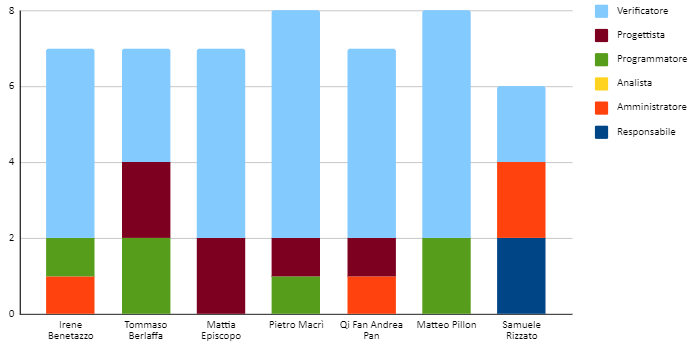
\includegraphics[width=\textwidth, height=\textheight, keepaspectratio]{images/preventivo/CA-obbligatori-orario.png}
    \caption{CA-validazione requisiti obbligatori - preventivo ripartizione oraria}
\end{figure}

\paragraph{Prospetto Economico}
\begin{center}
	\renewcommand{\arraystretch}{1.8} %aumento ampiezza righe
	\begin{tabular}{ |m{10em}|c|c|c|c|c|c|c| }
	\hline
	\textbf{Ruolo} & \textbf{Re} & \textbf{Am} &  \textbf{An} &  \textbf{Pt} &  \textbf{Pg} &  \textbf{Ve} &  \textbf{Totale}\\
    \hline
    Totale ore & 2 & 4 & 0 & 6 & 6 & 32 & \textbf{50}\\
    \hline
    Costo \euro/h & 30\euro/h & 20\euro/h & 25\euro/h & 25\euro/h & 15\euro/h & 15\euro/h & \\
    \hline
    \textbf{Totale costo} & \textbf{60\euro} & \textbf{80\euro} &  \textbf{0\euro} &  \textbf{150\euro} &  \textbf{90\euro} &  \textbf{480\euro} &  \textbf{860\euro}\\
    \hline
	\end{tabular}

\begin{figure}[H]
    \centering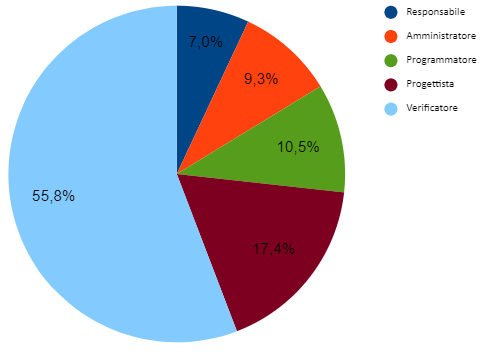
\includegraphics[scale=0.9]{images/preventivo/CA-obbligatori-costo.png}
    \caption{CA-validazione requisiti obbligatori - preventivo ripartizione economica}
\end{figure}
\end{center}

\newpage
\subsubsection{Validazione requisiti desiderabili}
\paragraph{Prospetto Orario}
\begin{center}
	\renewcommand{\arraystretch}{1.8} %aumento ampiezza righe
	\begin{tabular}{ |m{10em}|c|c|c|c|c|c|c| }
	\hline
	\textbf{Membro} & \textbf{Re} & \textbf{Am} &  \textbf{An} &  \textbf{Pt} &  \textbf{Pg} &  \textbf{Ve} &  \textbf{Totale}\\
    \hline
    Irene Benetazzo   & 2 & 2 & - & - & - & 3 & \textbf{7} \\
    \hline
    Tommaso Berlaffa  & - & 2 & - & - & - & 6 & \textbf{8} \\
    \hline
    Mattia Episcopo   & 1 & - & - & - & - & 4 & \textbf{5} \\
    \hline
    Pietro Macrì      & - & 2 & - & - & 2 & 5 & \textbf{9} \\
    \hline
    Qi Fan Andrea Pan & - & - & - & 3 & - & 6 & \textbf{9} \\
    \hline
    Matteo Pillon     & - & - & - & - & 1 & 5 & \textbf{6} \\
    \hline
    Samuele Rizzato   & - & - & - & 1 & 1 & 4 & \textbf{6} \\
    \hline
    \textbf{Totale ore} & \textbf{3} & \textbf{6} &  \textbf{0} &  \textbf{4} &  \textbf{4} &  \textbf{33} &  \textbf{50}\\
    \hline
	\end{tabular}
\end{center}
\begin{figure}[H]
    \centering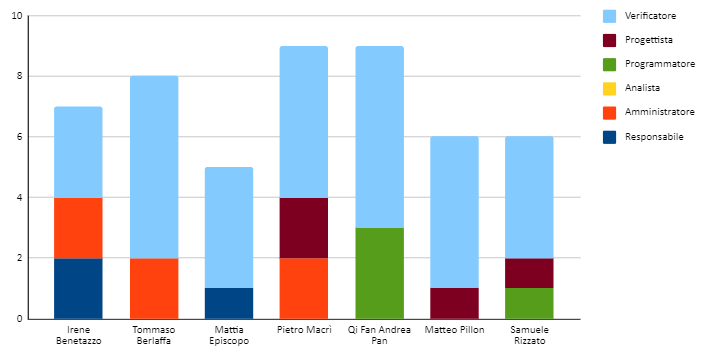
\includegraphics[width=\textwidth, height=\textheight, keepaspectratio]{images/preventivo/CA-desiderabili-orario.png}
    \caption{CA-validazione requisiti desiderabili - preventivo ripartizione oraria}
\end{figure}
\pagebreak
\paragraph{Prospetto Economico}
\begin{center}
	\renewcommand{\arraystretch}{1.8} %aumento ampiezza righe
	\begin{tabular}{ |m{10em}|c|c|c|c|c|c|c| }
	\hline
	\textbf{Ruolo} & \textbf{Re} & \textbf{Am} &  \textbf{An} &  \textbf{Pt} &  \textbf{Pg} &  \textbf{Ve} &  \textbf{Totale}\\
    \hline
    Totale ore & 3 & 6 & 0 & 4 & 4 & 33 & \textbf{50}\\
    \hline
    Costo \euro/h & 30\euro/h & 20\euro/h & 25\euro/h & 25\euro/h & 15\euro/h & 15\euro/h & \\
    \hline
    \textbf{Totale costo} & \textbf{90\euro} & \textbf{120\euro} &  \textbf{0\euro} &  \textbf{100\euro} &  \textbf{60\euro} &  \textbf{495\euro} &  \textbf{865\euro}\\
    \hline
	\end{tabular}

\begin{figure}[H]
    \centering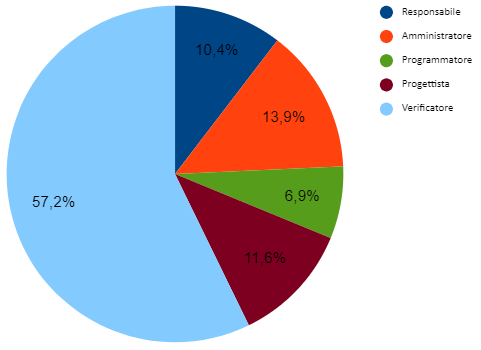
\includegraphics[scale=0.9]{images/preventivo/CA-desiderabili-costo.png}
    \caption{CA-validazione requisiti desiderabili - preventivo ripartizione economica}
\end{figure}
\end{center}


\newpage